\FloatBarrier
\begin{figure}[!h]
\centering
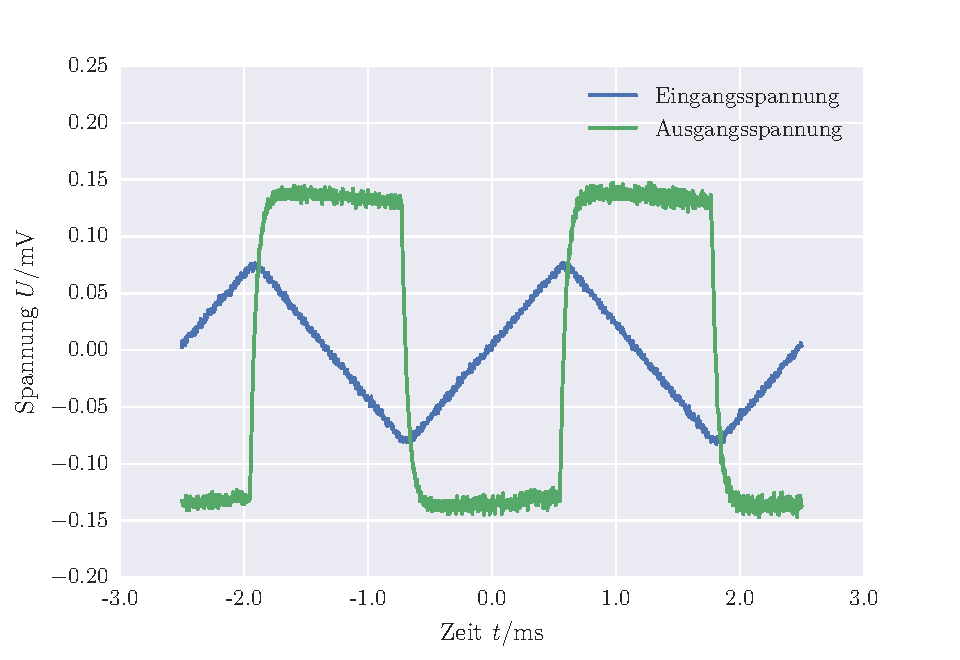
\includegraphics[scale=0.75]{../Grafiken/Differentiator_Oszilloskop_Dreieck.pdf}
\caption{Vom Oszilloskop aufgenommene Ein- und Ausgangsspannungen der Differentiatorschaltung. Auf dem Eingang
	liegt hier eine Dreiecksspannung.  Die Ausgangsspannung in Form einer Rechteckspannung entspricht dem theoretisch
	zu erwartendem Verlauf.\label{fig:differentiator_oszilloskop_dreieck}}
\end{figure}
\FloatBarrier